\section{Herleitung Initialgeschwindigkeit bei Kugel-Kollision}\label{anhang:herleitung:ballCollisionReverse}
Eine Kugel T soll in eine gewünschte Richtung rollen. Dazu soll sie von einer anderen Kugel A angestossen werden.
Gesucht ist der Punkt, wohin Kugel A rollen muss, um mit Kugel T zusammenzustossen.
Die Kugel T soll mit einer bestimmten Geschwindigkeit von der Kollision ausgehen.
Dazu ist die Geschwindigkeit zu bestimmen, die Kugel A  zum Zeitpunkt der Kollision haben muss.

Die Situation mit der Kugel T, an der Position $C$ und der Kugel A, an der Position $A$ ist in Abbildung \ref{fig:ballCollisionPointReverse_anhang}
dargestellt. Die Kugel A muss zum Punkt $B$ rollen, wo sie auf Kugel T prallt und ein elastischer Stoss\cite{wiki.elastischer_stoss_physik:1} stattfindet.
Während die Kugel die Distanz $\norm{\vec{d}}$ zurücklegt, verliert sie an Geschwindigkeit aufgrund von Reibung,
diese wird in Abschnitt \ref{ReibungsverlustUeberBahn} behandelt. Hier ist lediglich relevant, welche Geschwindigkeit
die Kugel A am Punkt $B$ haben muss.

\begin{figure}[h!]
    \begin{center}
        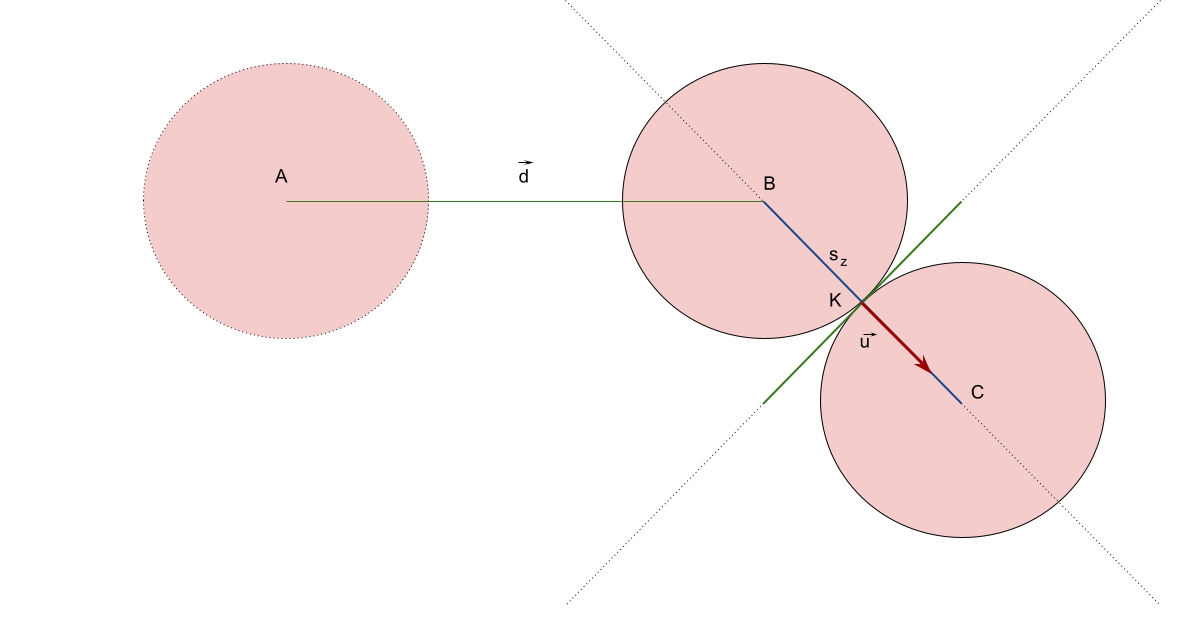
\includegraphics[width=0.6\linewidth]{../common/03_billiard_ai/resources/21_kollisionspunkt_rueckwaerts.png}
    \end{center}
    \caption{Kollisionspunkt zweier Kugeln}
    \label{fig:ballCollisionPointReverse_anhang}
\end{figure}

Sei die gewünschte Richtung, in die Kugel T nach der Kollision rollen soll, $\hat{u}$ und der Kugelradius $r$, dann kann die Position $B$ bestimmt werden:
\begin{align}
    s_z = 2 \cdot r\\
    B = C - s_z \cdot \hat{u}\\
    B = C - 2 \cdot r \cdot \hat{u}
\end{align}

Nun gilt es die Geschwindigkeit $\vec{v_{1,z}}$ der Kugel A zum Zeitpunkt der Kollision zu bestimmen.
Nachfolgend wird angenommen, dass die zu treffende Kugel T stillsteht und somit die Geschwindigkeit $\vec{v_2} = \vec{0}$ hat.
Der Geschwindkeitsvektor $\vec{u}$ ist durch die gewünschte Richtung und Geschwindigkeit,
welche die Kugel T nach dem Zusammenstoss haben soll, gegeben.
\begin{align}
    \vec{u} = \vec{v_{1,z}} + \vec{v_{2,t}}\\
    \vec{u} = \vec{v_{1,z}} + \vec{0}\\
    \vec{u} = \vec{v_{1,z}}
\end{align}
Die Situation ist in Abbildung \ref{fig:elasticCollisionOfTwoBalls} dargestellt.

\begin{figure}[h!]
    \begin{center}
        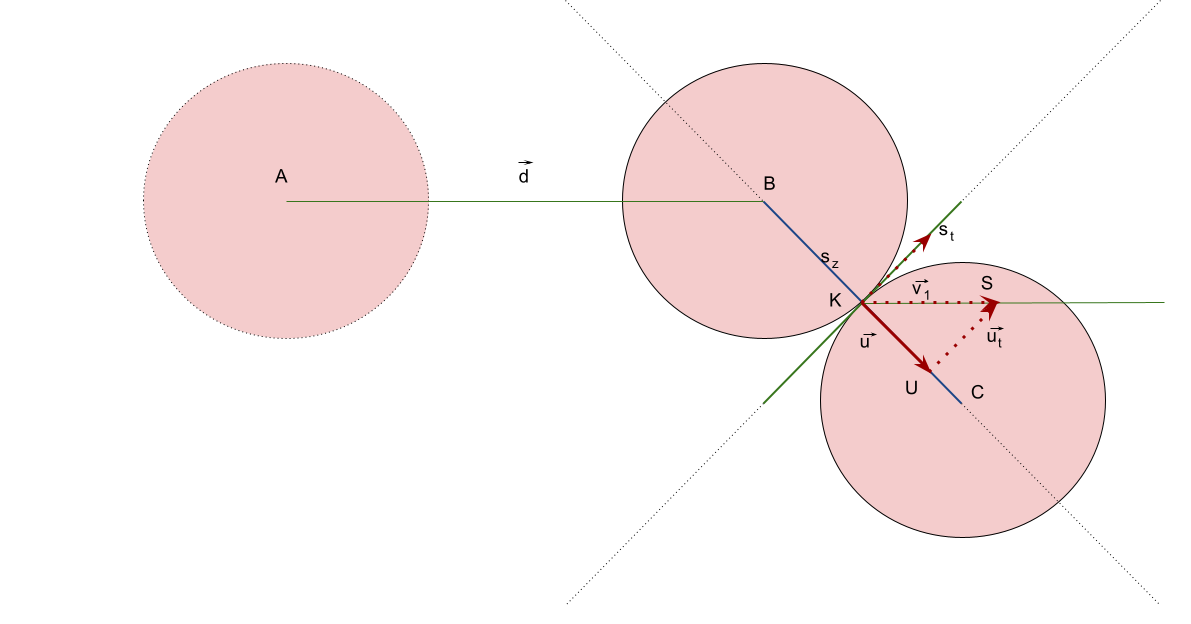
\includegraphics[width=0.6\linewidth]{../common/03_billiard_ai/resources/22_kollision_rueckwaerts.png}
    \end{center}
    \caption{Elastischer Stoss zweier Kugeln}
    \label{fig:elasticCollisionOfTwoBalls}
\end{figure}

Gegeben sind die nachfolgenden Informationen:
\begin{itemize}
    \item $A$: Startposition der Kugel A.
    \item $C$: Position der Kugel T.
    \item $\vec{u}$: Gewünschte Geschwindigkeit und Richtung der Kugel T nach dem Zusammenstoss.
\end{itemize}

Weiterhin ist die Richtung von $\vec{v_1}$ gegeben, da dieser parallel zum Vektor $\vec{d}$ ist.
Allerdings muss die Länge des Vektors noch bestimmt werden:
\begin{align}
    \vec{d} = B - A\\
    \hat{d} = \frac{\vec{d}}{\norm{\vec{d}}}\\
    \vec{v_1} = \alpha \cdot \hat{d}
\end{align}

Die Länge des Vektors $\vec{v_1}$ muss nach Projektion auf den Einheitsvektor $\hat{u}$ in Richtung
von $\vec{u}$ der Länge des Vektors $\vec{u}$ entsprechen. Dazu muss ein Skalierungsfaktor $\alpha$ bestimmt werden,
mit dem der Einheitsvektor $\hat{d}$ skaliert werden kann:
\begin{align}
    \hat{u} = \frac{\vec{u}}{\norm{\vec{u}}}\\
    \vec{v_1} \cdot \hat{u} = \norm{\vec{u}}\\
    (\alpha \cdot \hat{d}) \cdot \hat{u} = \norm{\vec{u}}\\
    \alpha \cdot (\hat{d} \cdot \hat{u}) = \norm{\vec{u}}\\
    \alpha = \frac{\norm{\vec{u}}}{\hat{d} \cdot \hat{u}}\\
    \alpha = \frac{\norm{\vec{u}}}{\hat{d} \cdot \frac{\vec{u}}{\norm{\vec{u}}}}\\
    \alpha = \frac{\norm{\vec{u}}^2}{\hat{d} \cdot \vec{u}}\\
    \alpha = \frac{\vec{u} \cdot \vec{u}}{\hat{d} \cdot \vec{u}}\\
    \vec{v_1} = \alpha \cdot \hat{d}\\
    \vec{v_1} = \frac{\vec{u} \cdot \vec{u}}{\hat{d} \cdot \vec{u}} \cdot \hat{d}
\end{align}

Somit ist die Geschwindigkeit, welche die Kugel A an Position B haben muss, bestimmt.
Der Energieverlust wird über eine Konstante $E_v$ definiert, welche in Prozent angegeben wird.
Es resultiert eine Verlängerung des berechneten Vektors.
\begin{align}
    \vec{v_1} = \frac{\vec{u} \cdot \vec{u}}{\hat{d} \cdot \vec{u}} \cdot \frac{1}{1 - E_v} \cdot \hat{d}
\end{align}